%% BioMed_Central_Tex_Template_v1.06
%%                                      %
%  bmc_article.tex            ver: 1.06 %
%                                       %


%%% additional documentclass options:
%  [doublespacing]
%  [linenumbers]   - put the line numbers on margins

%%% loading packages, author definitions

%\documentclass[twocolumn]{bmcart}% uncomment this for twocolumn layout and comment line below
\documentclass{bmcart}
%%% Load packages
\usepackage{amsthm,amsmath}
%\RequirePackage[numbers]{natbib}
%\RequirePackage[authoryear]{natbib}% uncomment this for author-year bibliography
%\RequirePackage{hyperref}
\usepackage{booktabs} %unicode support
\usepackage[utf8]{inputenc} %unicode support
%\usepackage[applemac]{inputenc} %applemac support if unicode package fails
%\usepackage[latin1]{inputenc} %UNIX support if unicode package fails
\usepackage{floatrow}
\floatsetup[table]{capposition=top}
%%%%%%%%%%%%%%%%%%%%%%%%%%%%%%%%%%%%%%%%%%%%%%%%%
%%                                             %%
%%  If you wish to display your graphics for   %%
%%  your own use using includegraphic or       %%
%%  includegraphics, then comment out the      %%
%%  following two lines of code.               %%
%%  NB: These line *must* be included when     %%
%%  submitting to BMC.                         %%
%%  All figure files must be submitted as      %%
%%  separate graphics through the BMC          %%
%%  submission process, not included in the    %%
%%  submitted article.                         %%
%%                                             %%
%%%%%%%%%%%%%%%%%%%%%%%%%%%%%%%%%%%%%%%%%%%%%%%%%

\usepackage{graphicx}
%\def\includegraphic{}
%\def\includegraphics{}
\graphicspath{ {media/} }
\usepackage{subcaption}
\captionsetup[subfigure]{width=0.9\textwidth}
%% Put your definitions there:
\startlocaldefs
\endlocaldefs

%%% Begin ...
\begin{document}
	
	%%% Start of article front matter
	\begin{frontmatter}
		
		\begin{fmbox}
			\dochead{Research}			
			\title{Impact of COVID-19 Pandemic on Perceived Access and Quality of Care in German People with Parkinson’s Disease}
			
			%%%%%%%%%%%%%%%%%%%%%%%%%%%%%%%%%%%%%%%%%%%%%%
			%%                                          %%
			%% Enter the authors here                   %%
			%%                                          %%
			%% Specify information, if available,       %%
			%% in the form:                             %%
			%%   <key>={<id1>,<id2>}                    %%
			%%   <key>=                                 %%
			%% Comment or delete the keys which are     %%
			%% not used. Repeat \author command as much %%
			%% as required.                             %%
			%%                                          %%
			%%%%%%%%%%%%%%%%%%%%%%%%%%%%%%%%%%%%%%%%%%%%%%
			
			\author[
			addressref={aff1},                   % id's of addresses, e.g. {aff1,aff2}
			%corref={aff1},                       % id of corresponding address, if any
			noteref={n1},                        % id's of article notes, if any
			email={marlena.vanmunster@uni-marburg.de}   % email address
			]{\inits{M.v.M.} \fnm{Marlena} \snm{van Munster}}
			\author[
			addressref={aff1},
			noteref={n1},
			email={marcel.printz@uni-marburg.de}
			]{\inits{M.P.} \fnm{Marcel} \snm{Printz}}
			\author[
			addressref={aff1, aff2},
			corref={aff1},                       % id of corresponding address, if any
			email={david.pedrosa@staff.uni-marburg.de}
			]{\inits{D.J.P} \fnm{David J.} \snm{Pedrosa}}
			
			%%%%%%%%%%%%%%%%%%%%%%%%%%%%%%%%%%%%%%%%%%%%%%
			%%                                          %%
			%% Enter the authors' addresses here        %%
			%%                                          %%
			%% Repeat \address commands as much as      %%
			%% required.                                %%
			%%                                          %%
			%%%%%%%%%%%%%%%%%%%%%%%%%%%%%%%%%%%%%%%%%%%%%%
			
			\address[id=aff1]{%                          	% unique id
				\orgdiv{Department of Neurology},             % department, if any
				\orgname{Philipps University},          % university, etc
				\city{Marburg},                              % city
				\cny{Germany}                                    % country
			}
			
			\address[id=aff2]{%                          	% unique id
				\orgdiv{Centre of Mind, Brain and Behaviour},             % department, if any
				\orgname{Philipps University},          % university, etc
				\city{Marburg},                              % city
				\cny{Germany}                                    % country
			}
			
			%%%%%%%%%%%%%%%%%%%%%%%%%%%%%%%%%%%%%%%%%%%%%%
			%%                                          %%
			%% Enter short notes here                   %%
			%%                                          %%
			%% Short notes will be after addresses      %%
			%% on first page.                           %%
			%%                                          %%
			%%%%%%%%%%%%%%%%%%%%%%%%%%%%%%%%%%%%%%%%%%%%%%
			
			\begin{artnotes}
			%\note{Sample of title note}     % note to the article
			\note[id=n1]{These authors contributed equally} % note, connected to author
			\end{artnotes}
			
		\end{fmbox}% comment this for two column layout
		
		%%%%%%%%%%%%%%%%%%%%%%%%%%%%%%%%%%%%%%%%%%%%%%%
		%%                                           %%
		%% The Abstract begins here                  %%
		%%                                           %%
		%% Please refer to the Instructions for      %%
		%% authors on https://www.biomedcentral.com/ %%
		%% and include the section headings          %%
		%% accordingly for your article type.        %%
		%%                                           %%
		%%%%%%%%%%%%%%%%%%%%%%%%%%%%%%%%%%%%%%%%%%%%%%%
		
		\begin{abstractbox}
			
			\begin{abstract} % The Abstract should not exceed 350 words. 
				\parttitle{Background} 
				the context and purpose of the study.
				\parttitle{Methods} 
				how the study was performed and statistical tests used
				\parttitle{Results} 
				the main findings.
				\parttitle{Conclusions} 
				brief summary and potential implications.
				\parttitle{Trial Registration} 
				If your article reports the results of a health care intervention on human participants, it must be registered in an appropriate registry and the registration number and date of registration should be in stated in this section. If it was not registered prospectively (before enrollment of the first participant), you should include the words 'retrospectively registered'.
			\end{abstract}
			
			%%%%%%%%%%%%%%%%%%%%%%%%%%%%%%%%%%%%%%%%%%%%%%
			%%                                          %%
			%% The keywords begin here                  %%
			%%                                          %%
			%% Put each keyword in separate \kwd{}.     %%
			%%                                          %%
			%%%%%%%%%%%%%%%%%%%%%%%%%%%%%%%%%%%%%%%%%%%%%%
			
			\begin{keyword}				%three to ten keywords
				\kwd{Parkinson's disease}
				\kwd{COVID-19 pandemic}
				\kwd{health care}
				\kwd{impact}
				\kwd{influence}
				\kwd{Germany}
				\kwd{iCARE-PD}
			\end{keyword}
			
			% MSC classifications codes, if any
			%\begin{keyword}[class=AMS]
			%\kwd[Primary ]{}
			%\kwd{}
			%\kwd[; secondary ]{}
			%\end{keyword}
			
		\end{abstractbox}
		%
		%\end{fmbox}% uncomment this for two column layout
		
	\end{frontmatter}
	
	%%%%%%%%%%%%%%%%%%%%%%%%%%%%%%%%%%%%%%%%%%%%%%%%
	%%                                            %%
	%% The Main Body begins here                  %%
	%%                                            %%
	%% Please refer to the instructions for       %%
	%% authors on:                                %%
	%% https://www.biomedcentral.com/getpublished %%
	%% and include the section headings           %%
	%% accordingly for your article type.         %%
	%%                                            %%
	%% See the Results and Discussion section     %%
	%% for details on how to create sub-sections  %%
	%%                                            %%
	%% use \cite{...} to cite references          %%
	%%  \cite{koon} and                           %%
	%%  \cite{oreg,khar,zvai,xjon,schn,pond}      %%
	%%                                            %%
	%%%%%%%%%%%%%%%%%%%%%%%%%%%%%%%%%%%%%%%%%%%%%%%%
	
	%%%%%%%%%%%%%%%%%%%%%%%%% start of article main body
	% <put your article body there>
	
	%%%%%%%%%%%%%%%%
	%% Background %%
	%%
	\section*{Background}
	The COVID-19 pandemic is an unprecedented event for people within the last few generations. The uncontrolled spread of a virus causing potential fatal side effects despite maximal intensive care therapies and the consecutive necessity to reduce everyday life has afflicted Western societies economically, culturally but obviously also within healthcare systems. In an attempt to spare societies from far worse, everyday world almost ceased with rising incidences rose and public access to almost all services was limited to the most basic needs, leaving those particularly exposed, who may not be vitally at harm but whose well-being may heyvily rely on intact social functioning.

People suffering from chronical illnesses attain more freqently to non-emergency medical services and were therefore at high risk of undersupply during the pandemic. Numerous studies have unveiled the impact of the COVID-19 pandemic on chronically-ill patients \cite{olivieri2021auswirkungen, ceglaeinfluss}. Yet, at the same time the need to remain at home has brought up many examples of solidarity but has also enabled societies to rapidly evolve in terms of remote medical solutions only hampered in their efficiency as not many validated tools existed before. In neurology, subjects particularly prone for undersupply were thos suffereing from neurodegenerative disease and particularly Parkinson's disease %Kann man das mit einer Quelle belegen?%. 

. had profound impact on the accesibility of medical services. In order to learn from the pandemic in the long term, difficulties in access to healthcare must be uncovered and addressed \cite(iyengar2020learning). Although numerous studies in Germany analyze %weiß nocht nicht so genau, wie ichb das einbringen würde. Ist aber wichtig!%


People with Parkinson's disease (PwP) suffer from a progressive condition showing a great heterogeneity. Motor, as well an non-motor symptoms may develop so that tailored treatment options and continuous adjustments are necessary. One may therefore infer, that restrictions of healthcare services may have striken those patients at a very high level. Surprisingly, only a limited number of studies have this far examined the impact of the COVID-19 pandemic on PwPs in Germany \cite{zipprich2020knowledge, frundt2022impact, richter2021analysis}. These studies focus on personal behaviour, knowledge and access to specialized therapies. A recent study by Fründt et al. investigated the impact of the pandemic on PwPs general healthcare situation with a specific focus on long-term care \cite{frundt2022impact} and contrary to one might expect posit that deficits in health care were less severe than expected \cite{frundt2022impact}. Given the good performance of the German healthcare system during the COVID-19 pandemic, these results do not come as surprise \cite{10665-341674}. %den Satz würde ich in die Diskussion packen%
	
	However, studies from other areas of public health research show, that the effect of public health crisis are not universal but affect some individuals more than others \cite{huijts2017prevalence, lowcock2012social}. This inequality can be explained by so-called  social determinants of health (SDH). SDH are non-medical factors that influence, among other things, peoples access to healthcare. The link between SDH and individuals access to healthcare is observable with regard to the COVID-19 pandemic, which means that some population groups experienced greater impacts than others based on their SDH \cite{whocovidbrief}.
	
	There are several conceptualizations and definitions of what SDH are but in a broadest sense, they compromise contextual, structural and individual factors \cite{world2010conceptual}. The word \textit{contextual} is of utmost importance here: what may be considered as relevant SDH is not universal. For the context of Parkinson's disease, Zaman  et al. proposed a model which summarizes structural and individual factors that may influence PwPs access to healthcare \cite{zaman2021barriers}. 
	Structural SDH in this model may be reflected by barrieres, that PwPs meet on a system-level when trying to access healthcare, such as a lack of care coordination, limited communication between healthcare providers, disparities in health services or the unavailability of specialit services \cite{zaman2021barriers}. Individual SDH may be reflected by personal barriers in this model, which influence the PwPs ability to seek help, engage with care providers, reach important care services or pay for them \cite{zaman2021barriers}. 
	
	To the best of our knowledge, it has not been investigated how SDH may explain the impact of the COVID-19 pandemic on PwPs access to healthcare. Therefore, we here explicitly examine the impact of relevant SDH on PwPs access to healthcare during the COVID-19 pandemic in Germany. The basis of our analysis is the German dataset of an anonymous survey that was carried out as part of the iCARE-PD project. In the iCARE-PD project, international collaborators are seeking ways to improve health care for PwP by establishing integrated care models. These models are characterized by a patient-centered approach with coordination of local healthcare providers and application of technology-based solutions \cite{fabbri2020moving}.  
	
\section*{Methods}
The survey developed in the iCARE-PD project was designed to characterize the access of PwP to health services and to identify barriers in order to develop solutions to overcome them in the future.  In addition, the impact of the Covid-19 pandemic on the care situation of Parkinson's patients was to be investigated.
The questionnaire consists of four parts. Part A was used to describe the patients' health status (in terms of their Parkinson's disease and concomitant diseases), and Part D was used to determine their demographic background. Part B contained questions about health care experiences in the last 12 months before the Covid-19 pandemic (for example, concerning existing personal resources, local availability of health care providers, barriers to accessing services, and satisfaction with care).  Part C addressed questions about experiences with health care during the Covid-19 pandemic and the use of telemedicine services.
The questionnaire included 49 questions. Some of them were to be answered only depending on previous answers. Single or multiple-choice questions and open-ended questions were used.
The questionnaire was originally developed in English and translated into German for use in Germany. %who did it with which program, if any?%.
The invitation to participate in the survey was sent via the e-mail distribution list of the German Parkinson Association (Deutsche Gesellschaft für Parkinson und Bewegungsstörungen, DPG) and was addressed to all patients with a doctor's diagnosis of Parkinson's disease. The questionnaire was available for anonymous and voluntary participation via the online platform SoSci Survey from November 2020 to January 2021. Participation was possible via a computer as well as by cell phone.
The study was approved by the local Ethics committee and carried out in accordance with the Declaration of Helsinki. The study is registered under the study ID DRKS00025764 in the German Clinical Trial Register. All patients gave informed written consent prior to participating. %In what way was the latter done in our online survey?%.
In addition to Germany, the questionnaire was also distributed in Canada, Spain, Portugal and the Czech Republic. In our evaluation, we limit ourselves to the data collected with the survey in Germany.
We received 551 answered questionnaires, of which 388 (70.4%) were completely filled out.
%What does complete mean and how were the data checked and transferred to the Excel spreadsheet?%.
In our analysis, in addition to the data from the survey, we also included information on the density of neurologists, general practitioners, and population according to zip code, which was available via %source of information%.
For the available data on comorbidities, we applied the Elixhäuser Comorbitiy Score modified by van Walraven \cite {van2009modification}.
%the following part is still under construction and please be checked%
We used R (version 4.1.1) to perform statistical analyses.
To test for significance of differences in the median of ordinal scaled variables (B17/C6), we used a sign test.
To examine the direction and strength of the influence of selected predictors on the manifestation of C4, we performed multiple and stepwise logistic regression with determination of odds ratios.
We made the selection of predictors to be examined based on previously characterized barriers to accessing health services regarding PwP\cite {zaman2021barriers}.

\subsection*{Participants}


\section*{Results}
In total, 552 questionnaires were filled out with 252 different postal codes. Further demographics are listed in Table~\ref{tab1:demographics}. With respect to the distribution of the questionnaires, participants were located at all regions in Germany (cf. Figure~\ref{fig1:questionnaires}

\begin{table}[!ht]
%\centering
\begin{tabular}{p{5cm} c}
\toprule
																	&	\textbf{Overall}	\\ %\hline
																	& 	\textbf{(n = 552)}\\ 
\midrule
Age (mean (SD)) 															& 	66.76 (9.25) 	\\ \hline
Gender = female (\%) 														&  	148 (41.6)  		\\ \hline
Disease duration (\%) 														& 				\\ \hline
\hspace{3mm} $<$2 years 													& 	62 (13.1) 		\\ \hline
\hspace{3mm} 2--5 years 													& 	154 (32.6) 		\\ \hline
\hspace{3mm} 5--10 years 													& 	157 (33.2) 		\\ \hline
\hspace{3mm} 10--15 years 													& 	69 (14.6) 		\\ \hline
\hspace{3mm} $>$15 years													& 	31 ( 6.6) 		\\ \hline
Disease stage (\%)														& 				\\ \hline
\hspace{3mm} Hoehn \& Yahr I 												&  	189 (40.3) 		\\ \hline
\hspace{3mm} Hoehn \& Yahr II 												& 	156 (33.3)  		\\ \hline
\hspace{3mm} Hoehn \& Yahr III  												&   	77 (16.4) 		\\ \hline
\hspace{3mm} Hoehn \& Yahr IV  												& 	41 ( 8.7) 		\\ \hline
\hspace{3mm} Hoehn \& Yahr V  												&     	6 ( 1.3) 		\\ \hline
Education level according \newline to ISCED (\%) 									& 				\\ \hline
\hspace{3mm} primary education  												& 	20 ( 5.0) 		\\ \hline
\hspace{3mm} secondary education 						 					& 	234 (58.4)		\\ \hline
\hspace{3mm} post secondary education  										&   	69 (17.2) 		\\ \hline
\hspace{3mm} highest education level possible 										& 	78 (19.5)  		\\ \hline
\hspace{3mm} PDQ-8 scores (mean (SD)) 										& 	41.30 (14.23) 	\\ \hline
Van-Walraven-Elixhauser \newline \hspace{3mm} Comorbidity Index (mean (SD)) 	& 	6.55 (1.95) 		\\ 
\bottomrule
\caption{Demographics of subjects filling out questionnaire:}
\label{tab1:demographics}
\end{tabular}
\end{table}

\begin{figure}
    \centering
    \begin{subfigure}[b]{0.35\linewidth}
        \includegraphics[width=.90\textwidth]{"available.questionnaires".jpeg}
        \caption{Available questionnaires for this project}
        \label{fig1:questionnaires}
    \end{subfigure}%
    \begin{subfigure}[b]{0.35\linewidth}
        \includegraphics[width=.90\textwidth]{"population.perskmGER".jpeg}
        \caption{Inhabitants per square kilometer, source: https://www.destatis.de}
        \label{fig1:population}
    \end{subfigure}%
    \begin{subfigure}[b]{0.35\linewidth}
        \includegraphics[width=.90\textwidth]{"neurologists.10122021".jpeg}
        \caption{Density of neurologists in Germany (source: https://www.kbv.de/html/)}
        \label{fig1:neurologists}
    \end{subfigure}%
\end{figure}

One of our primordial analyses, was to analyze how the satisfaction with PD-related care had evolved during the pandemic. For that purpose we asked the participants,$?$ %bitte ergänzen % 
A sign-test thereby indicated significantly lower values during the pandemic (Mdn = 1) compared to before (Mdn= 3, \textit{p} = 10\textsuperscript{-73}). More than 90\% of the participants thereby indicated to be "rather unsatisfied" or "very unsatisfied" with their PD-related care during the pandemic (cf Figure \ref{fig2:satisfaction}).

\begin{figure}
\centering
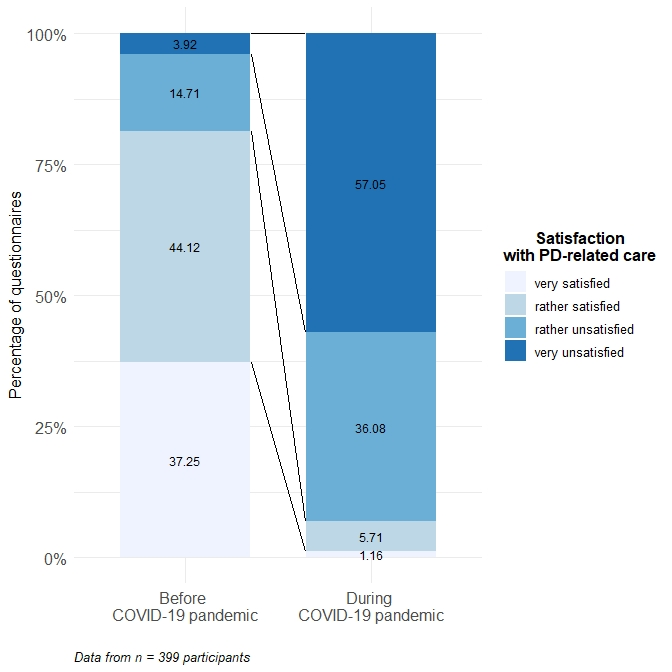
\includegraphics[width=.90\textwidth]{fig2.satisfaction.care.v1.0.jpeg}
\caption{Available questionnaires for this project}
\label{fig2:satisfaction}
\end{figure}

 Consecutively, for we could identify a series of predictors that significantly increased the odds that patinets affirmed the question that healthcare services would have been needed but were necessities were not met during the pandemic. HIgh significance was encountered for the factors: perceived expertise of the neurologist, the lack of ability to access PD-care before the pandemic, the experienced stigmatisation in healthcare, difficulties to acess healthcare services before the pandemic and the lack of PD-related care before the pandemic (all p $<$ .001). A graphic overview for significant predictors can be encountered in Figure \ref{fig3:resultsOR1} and the entire list of results is summarised in the supplementary material. % LInk einfügen.

\begin{figure}
\centering
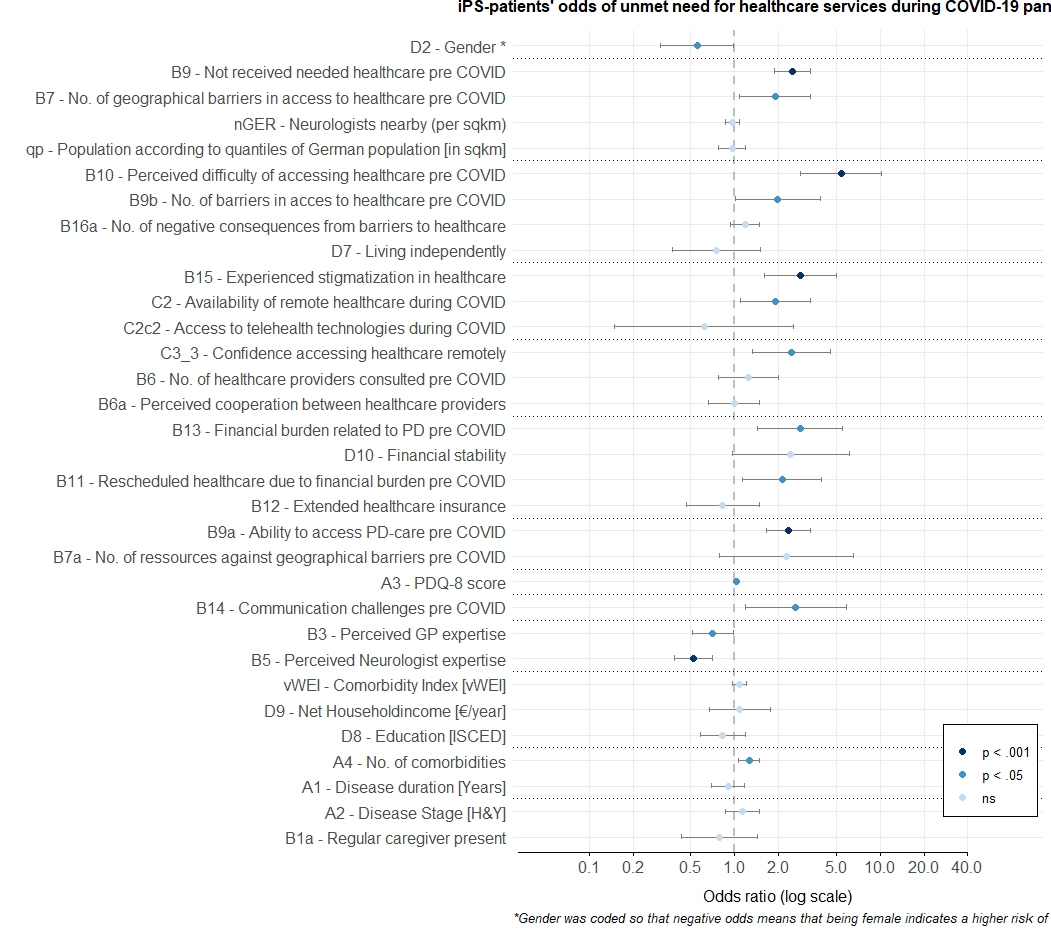
\includegraphics[width=.90\textwidth]{fig3.oddsratios.v1.0.jpeg}
\caption{Unadjusted Odds ratios according to the \textsc{GLM} for all 32 questions. Odds were determined so that higher values indicate affirmation to the question that healthcare was needed but this need remianed unmet during the COVID-19 pandemic. The dashed lines indicate the distinct domains according to ??, whereas significance is illustrated as color of the dot, with two distinct levels of significance. }%Quelle einfügen}
\label{fig3:resultsOR1}
\end{figure}


	\section*{Discussion}
	Text for this section\ldots
	\section*{Conclusion}
	Text for this section\ldots
	\subsection*{Sub-heading for section}
	Text for this sub-heading\ldots
	\subsubsection*{Sub-sub heading for section}
	Text for this sub-sub-heading\ldots
	\paragraph*{Sub-sub-sub heading for section}
	Text for this sub-sub-sub-heading\ldots
	
	In this section we examine the growth rate of the mean of $Z_0$, $Z_1$ and $Z_2$. In
	addition, we examine a common modeling assumption and note the
	importance of considering the tails of the extinction time $T_x$ in
	studies of escape dynamics.
	We will first consider the expected resistant population at $vT_x$ for
	some $v>0$, (and temporarily assume $\alpha=0$)
	%
	\[
	E \bigl[Z_1(vT_x) \bigr]=
	\int_0^{v\wedge
		1}Z_0(uT_x)
	\exp (\lambda_1)\,du .
	\]
	%
	If we assume that sensitive cells follow a deterministic decay
	$Z_0(t)=xe^{\lambda_0 t}$ and approximate their extinction time as
	$T_x\approx-\frac{1}{\lambda_0}\log x$, then we can heuristically
	estimate the expected value as
	%
	\begin{equation}\label{eqexpmuts}
		\begin{aligned}[b]
			&      E\bigl[Z_1(vT_x)\bigr]\\
			&\quad      = \frac{\mu}{r}\log x
			\int_0^{v\wedge1}x^{1-u}x^{({\lambda_1}/{r})(v-u)}\,du .
		\end{aligned}
	\end{equation}
	%
	Thus we observe that this expected value is finite for all $v>0$ (also see \cite{koon,xjon,marg,schn,koha,issnic}).
	
	
	\section*{Appendix}
	Text for this section\ldots
	
	%%%%%%%%%%%%%%%%%%%%%%%%%%%%%%%%%%%%%%%%%%%%%%
	%%                                          %%
	%% Backmatter begins here                   %%
	%%                                          %%
	%%%%%%%%%%%%%%%%%%%%%%%%%%%%%%%%%%%%%%%%%%%%%%
	
	\begin{backmatter}
		
		\section*{Acknowledgements}%% if any
		Text for this section\ldots
		
		\section*{Funding}%% if any
		Text for this section\ldots
		
		\section*{Abbreviations}%% if any
		Text for this section\ldots
		
		\section*{Availability of data and materials}%% if any
		Text for this section\ldots
		
		\section*{Ethics approval and consent to participate}%% if any
		Text for this section\ldots
		
		\section*{Competing interests}
		The authors declare that they have no competing interests.
		
		\section*{Consent for publication}%% if any
		Text for this section\ldots
		
		\section*{Authors' contributions}
		Text for this section \ldots
		
		\section*{Authors' information}%% if any
		Text for this section\ldots
		
		%%%%%%%%%%%%%%%%%%%%%%%%%%%%%%%%%%%%%%%%%%%%%%%%%%%%%%%%%%%%%
		%%                  The Bibliography                       %%
		%%                                                         %%
		%%  Bmc_mathpys.bst  will be used to                       %%
		%%  create a .BBL file for submission.                     %%
		%%  After submission of the .TEX file,                     %%
		%%  you will be prompted to submit your .BBL file.         %%
		%%                                                         %%
		%%                                                         %%
		%%  Note that the displayed Bibliography will not          %%
		%%  necessarily be rendered by Latex exactly as specified  %%
		%%  in the online Instructions for Authors.                %%
		%%                                                         %%
		%%%%%%%%%%%%%%%%%%%%%%%%%%%%%%%%%%%%%%%%%%%%%%%%%%%%%%%%%%%%%
		\section*{References}
		% if your bibliography is in bibtex format, use those command
		
		\bibliographystyle{vancouver} % Style BST file (bmc-mathphys, vancouver, spbasic).
		\bibliography{bmc_article_covidPD}      % Bibliography file (usually '*.bib' )
		
		%%%%%%%%%%%%%%%%%%%%%%%%%%%%%%%%%%%
		%%                               %%
		%% Figures                       %%
		%%                               %%
		%% NB: this is for captions and  %%
		%% Titles. All graphics must be  %%
		%% submitted separately and NOT  %%
		%% included in the Tex document  %%
		%%                               %%
		%%%%%%%%%%%%%%%%%%%%%%%%%%%%%%%%%%%
		
		%%
		%% Do not use \listoffigures as most will included as separate files
		
		\section*{Figures}
		\begin{figure}[h!]
			\caption{Sample figure title}
		\end{figure}
		
		\begin{figure}[h!]
			\caption{Sample figure title}
		\end{figure}
		
		%%%%%%%%%%%%%%%%%%%%%%%%%%%%%%%%%%%
		%%                               %%
		%% Tables                        %%
		%%                               %%
		%%%%%%%%%%%%%%%%%%%%%%%%%%%%%%%%%%%
		
		%% Use of \listoftables is discouraged.
		%%
		\section*{Tables}
		\begin{table}[h!]
			\caption{Sample table title. This is where the description of the table should go}
			\begin{tabular}{cccc}
				\hline
				& B1  &B2   & B3\\ \hline
				A1 & 0.1 & 0.2 & 0.3\\
				A2 & ... & ..  & .\\
				A3 & ..  & .   & .\\ \hline
			\end{tabular}
		\end{table}
		
		%%%%%%%%%%%%%%%%%%%%%%%%%%%%%%%%%%%
		%%                               %%
		%% Additional Files              %%
		%%                               %%
		%%%%%%%%%%%%%%%%%%%%%%%%%%%%%%%%%%%
		
		\section*{Additional Files}
		\subsection*{Additional file 1 --- Sample additional file title}
		Additional file descriptions text (including details of how to
		view the file, if it is in a non-standard format or the file extension).  This might
		refer to a multi-page table or a figure.
		
		\subsection*{Additional file 2 --- Sample additional file title}
		Additional file descriptions text.
	\end{backmatter}
\end{document}
